\section{Evaluation Workflow and Fault Model}\label{sec:fault}
The evaluation has three stages (Fig.~\ref{fig:workflow}). It freezes a trained model, its numerical execution and its task data. It builds protection masks from calibration data. It then compares those masks under common random faults. All clean and faulted outcomes come from the quantized executable itself, not from the differentiable companion model used to compute gradient scores. NetSuRF is the software implementation of this workflow; it is not a ranking in the comparison.

\begin{figure}[t]
\centering% Vector artwork: scientific workflow, with construction/evaluation boundary.
\begingroup%
\definecolor{flowink}{HTML}{17324D}%
\definecolor{flowteal}{HTML}{167D8D}%
\definecolor{flowblue}{HTML}{EEF4F8}%
\definecolor{flowgold}{HTML}{B36B25}%
\resizebox{\linewidth}{!}{%
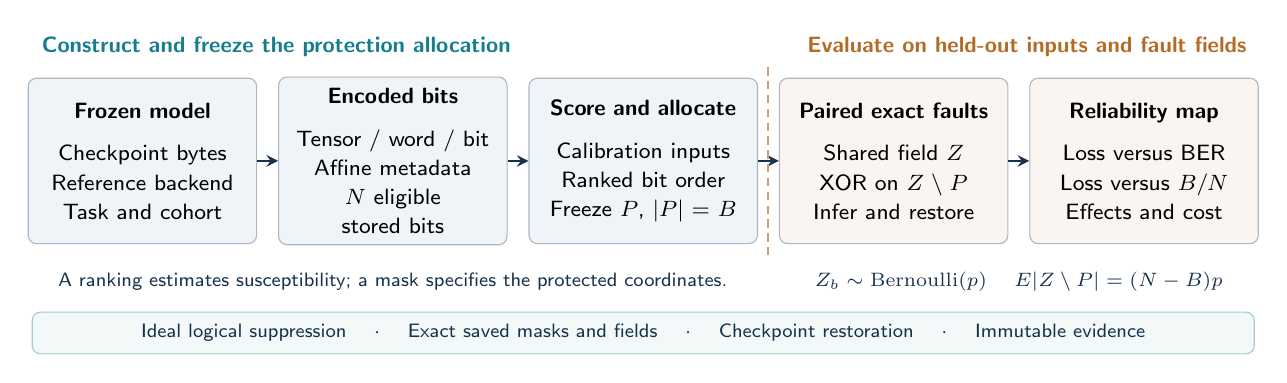
\begin{tikzpicture}[font=\sffamily\fontsize{8.5}{10.5}\selectfont,>=stealth,
  stage/.style={draw=flowink!35,fill=flowblue,rounded corners=3pt,
    minimum width=2.80cm,minimum height=2.10cm,text width=2.62cm,align=center,
    inner sep=4pt},
  edge/.style={->,draw=flowink,line width=0.85pt}]
\node[anchor=west,font=\sffamily\bfseries\footnotesize,text=flowteal] at (-1.4,1.45)
  {Construct and freeze the protection allocation};
\node[anchor=west,font=\sffamily\bfseries\footnotesize,text=flowgold] at (8.32,1.45)
  {Evaluate on held-out inputs and fault fields};
\node[stage] (model) at (0,0)
  {\textbf{Frozen model}\\[5pt]Checkpoint bytes\\Reference backend\\Task and cohort};
\node[stage] (bits) at (3.18,0)
  {\textbf{Encoded bits}\\[5pt]Tensor / word / bit\\Affine metadata\\$N$ eligible stored bits};
\node[stage] (mask) at (6.36,0)
  {\textbf{Score and allocate}\\[5pt]Calibration inputs\\Ranked bit order\\Freeze $P$, $|P|=B$};
\node[stage,fill=flowgold!7] (fault) at (9.54,0)
  {\textbf{Paired exact faults}\\[5pt]Shared field $Z$\\XOR on $Z\setminus P$\\Infer and restore};
\node[stage,fill=flowgold!7] (result) at (12.72,0)
  {\textbf{Reliability map}\\[5pt]Loss versus BER\\Loss versus $B/N$\\Effects and cost};
\draw[edge] (model)--(bits);
\draw[edge] (bits)--(mask);
\draw[edge] (mask)--(fault);
\draw[edge] (fault)--(result);
\draw[flowgold!65,densely dashed,line width=0.7pt] (7.95,-1.20)--(7.95,1.26);
\node[align=center,text=flowink,font=\sffamily\scriptsize] at (3.18,-1.53)
  {A ranking estimates susceptibility; a mask specifies the protected coordinates.};
\node[align=center,text=flowink,font=\sffamily\scriptsize] at (11.13,-1.53)
  {$Z_b\sim\mathrm{Bernoulli}(p)$ \quad $\mathbb{E}|Z\setminus P|=(N-B)p$};
\draw[draw=flowteal!40,fill=flowteal!5,rounded corners=3pt]
  (-1.40,-2.45) rectangle (14.12,-1.92);
\node[text=flowink,font=\sffamily\scriptsize] at (6.36,-2.185)
  {Ideal logical suppression \quad $\cdot$ \quad Exact saved masks and fields \quad $\cdot$ \quad Checkpoint restoration \quad $\cdot$ \quad Immutable evidence};
\end{tikzpicture}%
}%
\endgroup%

\caption{Evaluation workflow. A ranking orders bits, a mask fixes which bits are protected at a budget, and a fault field proposes random flips; the three are separate objects. Masks are frozen before paired evaluation. Protection cost counts bits; physical correction circuits are outside the study.}
\Description{Frozen model and bit identities lead to calibration-based rankings, fixed protection masks, paired exact faults and task-level reliability measurements.}
\label{fig:workflow}
\end{figure}

\paragraph{Eligible population.} The eligible population contains the $N$ bits of the stored INT8 weight codes: convolution and dense kernels in the TFLite models, and the weight matrices of all linear layers in the transformers. Each bit is identified by tensor, word and position; position zero is least significant and position seven is the sign bit. Zero-valued weights remain eligible. Biases, quantization scales and zero points, input embedding tables, normalization parameters and activations are not faulted (Appendix~\ref{app:implementation} lists them per model). They are therefore treated as perfectly reliable at no cost, which is an assumption of the study, not a finding.

\paragraph{Faults.} A fault XORs one stored bit. For example, code $5$ with scale $1/16$ represents $0.3125$; flipping its sign bit gives code $-123$, or $-7.6875$, an exact jump of $-8$. Several flips compose by XOR, but their task effects need not add.

\paragraph{Fields and masks.} A \emph{fault field} $Z$ proposes a flip at each eligible bit independently with probability $p$, the logical BER. A \emph{protection mask} $\protset$ contains $B$ protected bits and is chosen before evaluation. Only proposed flips outside the mask are applied: $A=Z\setminus\protset$. Protection suppresses events; it does not change which events are proposed. The same field is evaluated against every mask, held fixed over the whole input cohort, and removed before the next field. With $\risk(A)$ the task risk after applying $A$, the quantity compared at a fixed budget is
\begin{equation}\label{eq:expected-risk}
J_p(\protset)=\E_Z[\risk(Z\setminus\protset)].
\end{equation}
Coverage is $B/N$, and the expected numbers of proposed and applied faults are $Np$ and $(N-B)p$. Equal BER therefore means very different fault counts across models: at $p=10^{-5}$ ResNet-8 receives about six faults per field and Qwen3-0.6B about 48{,}000.
